\documentclass[journal]{IEEEtran}

% correct bad hyphenation here
\hyphenation{op-tical net-works semi-conduc-tor}
\usepackage{graphicx}

\begin{document}

\title{Sensor Descriptive Movements for Localization}

\author{Zheng~Lu,
        Zhiyang~Zhang,
        and~Michael~Craze
\thanks{Z. Lu, Z. Zhang and M. Craze is with the Department
of Electrical Engineering and Computer Science, University of Tennessee, Knoxville,
TN, 37996 USA }} 

% The paper headers
\markboth{Final Project Report for Class ECE555, November~2012}%
{Shell \MakeLowercase{\textit{et al.}}: Intros to SDM}

\IEEEspecialpapernotice{(Invited Paper)}

\maketitle

\begin{abstract}
Currently smartphone apps using GPS as their major source to acquire users' location. 
Due to the limitation of GPS in terms of energy efficiency and latency to fix a position, such apps will drain the battery in one or two hours and can hardly get responsive localization result. 
With the motivation of finding new ways to take advantage of sensors to improve our daily life, we propose to use sensors on modern smartphones to assist to keep track the movements of users to get better performance in localization applications. 
It is expected that by using sensors we can greatly reduce the usage of energy consuming GPS transceivers and can realize some location related applications with tight time constraints. 
We have then illustrated two possible applications which can take advantage of sensor data to describe user movements.
We focus on path recording application in this paper.
\end{abstract}

\begin{IEEEkeywords}
Sensors, Movement monitoring, Tracking, Smartphones
\end{IEEEkeywords}

\section{Introduction}
\IEEEPARstart {D}{ue} to the fast development of sensor technologies and the world wide spread of smartphones, more and more sensors have been integrated into our smartphones nowadays. 
These sensors enable us to realize many brand new applications which can greatly make our daily life more fruitful. 
Our location information is crucial for some applications these days, they may provide more specialized informations based on your location, such as route to a specific places, your path recordings of a travel. 
In this paper, we are going to propose a novel approach to provide location information.

\subsection{Why not use the GPS?}
GPS and its variance take advantage of GPS satellites to provide high precision localization information \cite{GPS}. 
A GPS receiver which can receive broadcast signals from GPS satellites is usually very cheap nowadays. 
Thus it is widely integrated into smartphones and used as major approach to get users' location. 

But there are several drawbacks of GPS, the first is that since it is a communication based approach, it will consume a lot of energy during localization. 
Since most embedded systems have very limited energy, this disadvantage makes it less practically in current embedded systems.
The second is that usually the startup performance is not very promising (as long as 12 minutes for regular GPS and dozens of seconds for A-GPS) \cite{A-GPS}, which means once you lose GPS signal, you will need a quiet long time to get your location again. 
This disadvantage makes it less possible to use GPS in some tightly time-constrianed applications. 

\subsection{How about the sensors?}
To reduce those disadvantages brought by GPS, we propose using sensors to describe human movements to help in acquiring location informations. 
Currently, most smartphones are equipped with sensors such as accelerometers, magnetometers and gyroscopes, which are capable of describing movement. 
By periodically monitoring these sensors and coordinately interpreting their readings, we can describe our movements with a acceptable accuracy. 
Once we get the movement description of users, we can calculate their current location together with their initial location which should be acquired though GPS or even manually set. 
Through this approach, we can minimize the usage of GPS to save energy or even implement some applications which have restrict time requirement that GPS cannot meet. 

The rest of the paper is organized as follows.
We will discuss two possible applications in Section II.
We study the measurements of energy consumption of GPS and sensors, as well as sensor readings to analyze advantage of sensor based localization in Section III.
Section IV provides the system overview of path recording application.

\section{Possible Applications}
We have proposed 2 specific sample applications here.

\begin{figure}
	\centering
	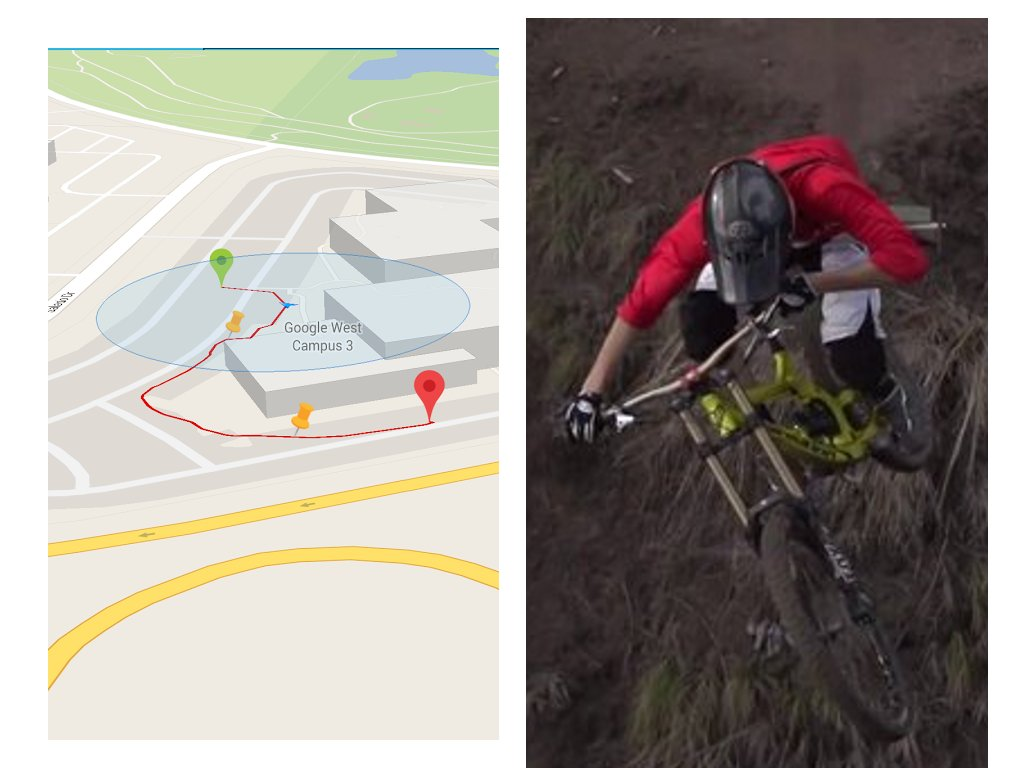
\includegraphics[width=3.5in]{figures/pic}
	\caption{(a) Path Recording Applications	(b) Personal Aerial Photography}
\end{figure}

\subsection{Personal aerial videotaping}
We emphasis on low latency to meet the restrict time constraints of applications. These applications can hardly be implemented by only using GPS, please refer to Fig.1 (b) .

\subsection{Path recording}
We emphasis on energy efficiency compared to regular GPS based path recording applications such as Google's "My tracks", please refer to Fig.1 (a) . 
The key idea in this application is that we will trying to use sensor readings to decide the best time of turning on GPS, while the GPS is off during most of the time.
Our goal is to reduce the turning on time of GPS as much as possible, so that more energy is saved. 

We will focus on this application in our following work. 

\section{The Measurements}
To verify the feasible and effective of our approach, we will study the energy consumption of GPS and sensors, as well as data readings from sensors.
For the specific application of path recording, we will also discuss some possible auxiliary means to increase our accuracy without sacrificing energy efficiency.

\begin{figure}
	\centering
	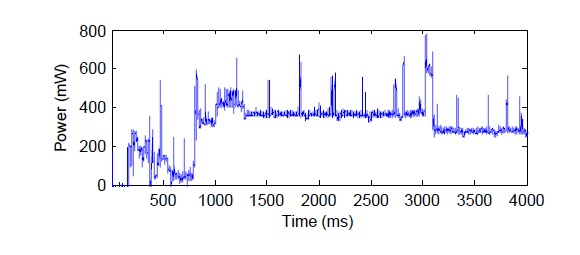
\includegraphics[width=3.5in]{figures/dpower}
	\caption{Detailed GPS power \cite{GPS Measurements} }
	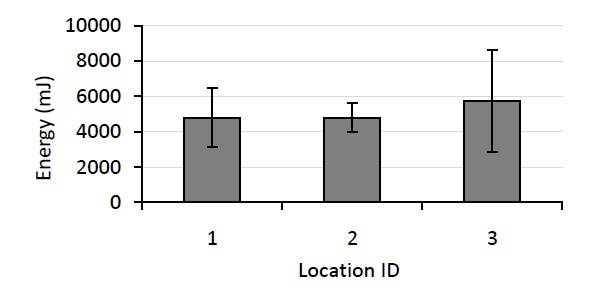
\includegraphics[width=3.5in]{figures/csenergy}
	\caption{GPS cold start energy consumption of different locations \cite{GPS Measurements} }
\end{figure}

\subsection{Energy consumption}
Before we trying to reduce energy consumption by replacing GPS with sensors as long as possible, we need to study the potential benefit of this method. 
This section study the energy consumption of GPS and sensors on smart phone to draw the potential energy saving of this approach. 

\subsubsection{Energy consumption of GPS} 
Reference \cite{GPS Measurements} gives a detailed measurement of energy consumption of GPS on Android smart phones. 
The power draw of GPS on android system has been measured at around 230mW compared to 324mW on Nokia N95. 
Please refer to Fig.2 for detailed energy consumption of GPS. 
Also, the energy consumption of GPS system varies when measure from different locations.
Fig.3 shows the energy measurements of a cold start of GPS in different locations.
We can draw from Fig.3 that by using A-GPS, the cold start up time is around 25 seconds.
Note that the energy consumption will drop to one forth when using a warm starts, that is, system has previous almanac or ephemeris data. 
Also, the warm start up time will be only around 6 seconds. 

\subsubsection{Energy consumption of sensors} 
While GPS cost large amount of energy, on the contrary, the sensors in smart phone requires far less energy. 
Using iPhone 5s's accelerometer chip STMicroelectronics LIS331DLH as an example \cite{Acc Measurements}. 
Under 2.5v supply voltage, the current consumption under normal mode is only 250uA and under low-power mode, this value is decreasing surprisingly to only 10uA. 
This means that the power consumption of this accelerometer is less than 1mW, negligible compared to power consumption of GPS. 

\subsubsection{Energy consumption of our approach} 
The sensor is absolutely more attractive with regards to energy consumption according to energy measurements above. 
In our implementation, we are considering using GPS signal discontinuously and using sensor readings to aid the locating when GPS is off. 
It is economic if we can always using warm start up after the first start. The minimal interval for us to turn on GPS should be larger than the warm start up time, that is, 6 seconds on average.
Also, according to the detailed energy consumption in Fig.2, GPS do not consume much more energy at start up than stable state. 
So, we can turn it off arbitrarily without facing any punishment in terms of energy consumption, but we may face a latency averaged at 6s when we trying to get location from GPS.
To conclude, the energy consumption of our method for locating is dominant by the power on time of GPS.

\subsection{Characteristic of sensor readings}
In this section, we design a simple test to study whether the characteristic of sensor readings are suitable for our tracking purpose.
During the test, we wrote a script running on a android smartphone to periodically recording accelerometer and magnetometer readings. 
We put the smartphone into the left pocket of pants and walking along a sidewalk.
We take two turns during the walking.

\begin{figure}
	\centering
	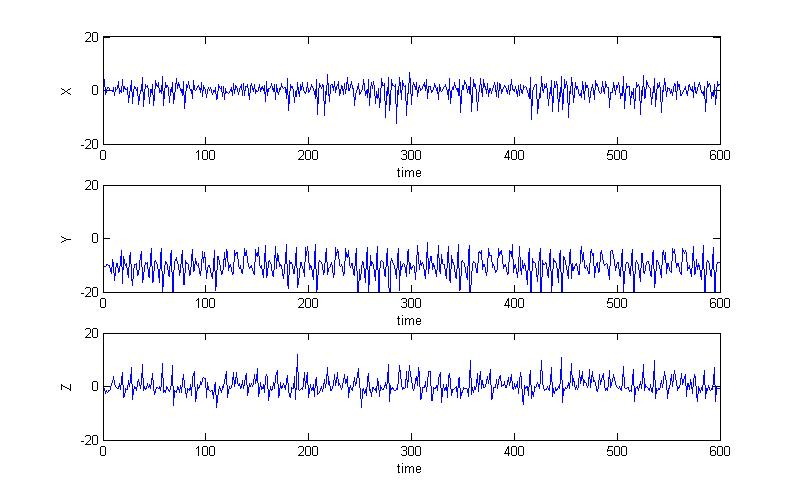
\includegraphics[width=3.5in]{figures/AccTest}
	\caption{Accelerometer readings of xyz coordinate system during the test}
	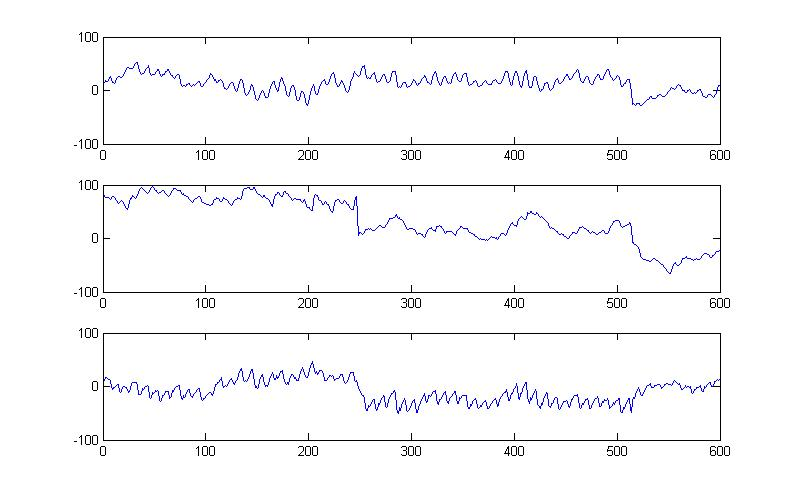
\includegraphics[width=3.5in]{figures/MagTest}
	\caption{Magnetometer readings of xyz coordinate system during the test}
\end{figure}

\subsubsection{Characteristic of accelerometer readings} 
The result seems chaos at the first look, but when we look into it, we may draw some really useful informations:

\begin{itemize}
	\item orientation of smartphone: 
		we can estimate the orientation of the cell phone, since the y axis is always around minus 10, which means that is the gravity.
	\item orientation of moving: 
		since in most of the time, the sensor readings of y axis and z axis is near symmetric of its mean value, we can learn that the person carrying the smartphone is moving along the x axis.
	\item direction of moving: 
		since the value is larger towards the minus direction of x axis, which means that we are approximately moving towards the minus x axis direction.
\end{itemize}

\subsubsection{Characteristic of magnetometer readings} 
The readings of magnetometer has more obvious trends compared to readings of accelerometer. 
We can draw the following information from its readings (note that the accelerometer and magnetometer are not necessarily share the same coordinate system):

\begin{itemize}
	\item orientation of smartphone: 
		we can estimate the orientation of the smartphone, this can help us using accelerometer and magnetometer cooperatively to more precisely determine the orientation of smartphone.
	\item orientation of turnings: 
		more interesting result from the magnetometer readings is that we can tell the direction of our turnings with these readings. 
		We are turning two times in this test scenario, you can find obvious clue of this two turning especially from y axis.
\end{itemize}

From above results and analysis, we can conclude from this experiment that we can draw sufficient information from sensor readings to describe our movements and assist localization when GPS is off. 

Although, we can also see that, since the sensor readings are suffering from volatiles because of the nature of our moving pattern, we can not calculate accurate movements and locations though these sensor readings.
So the GPS is still necessary for precise path recording of our approach.

\subsection{An auxiliary method to improve accuracy}
The google map on android system provides a function called geocoding, which we can use the coordinations we have to get the information of the road. 
So when we use the path recording application in city scenario, we can define our location result on the road.
This method can reduce the effect of volatile of sensor readings to the accuracy of the localization without incurring large energy consumption compared to acquiring location from GPS.

\section{System Overview}
Our goal is to deliver a low energy consumption, real-time accurate path recording system.
We will split our system into four parts according to their functionality, namely central controller, sensor data interpreter, map integrater, GPS coordinator.

\begin{figure}
	\centering
	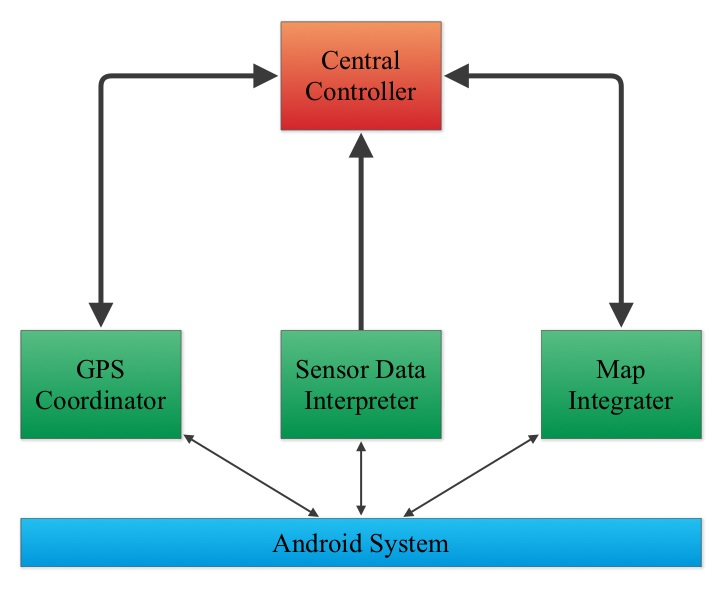
\includegraphics[width=3.5in]{figures/sysArc}
	\caption{System Architecture}
\end{figure}

\subsection{Non-functional requirements}
We will talk about the most important non-functional requirements in this section:

\begin{itemize}
	\item low power: 
		The major concern of our system is its power consumption. That is the main reason we sacrifice simplicity of only using GPS.
	\item real-time: 
		Since sensors do not suffering from high energy localization refresh overhead and long latency due to poor connection. 
		So we are expecting that our approach outperforms those only using GPS in terms of real-time in some scenarios such as urban areas, forests.
	\item accuracy: 
		The most significant drawback of sensor approach is its poor accuracy. 
		Although we can always increase the frequency of using GPS to achieve a better accuracy, this will reduce the benefit of our approach.
		We hope we can overcome low accuracy issue through better sensor readings interpreting algorithm design.
\end{itemize}

\subsection{System Components}
We will talk about the functionality of each component in our system.

\subsubsection{Central controller}
The central controller is where we keep the main logic of our system. 
Other components are all connected to this component. 
The central controller will monitor the possible localization errors in our algorithm by combining movement descriptions from  sensor data interpreter component and map auxiliary information from map integrater.
It will also determine the frequency of using GPS.
This component will also provide the user interface.

\subsubsection{Sensor data interpreter}
This is the major part of our system. 
It contains the algorithm of interpreting the sensor readings into movement descriptions. 
It will provide this informations to central controller.

\subsubsection{Map integrater}
This component has two functions. 
The first is to recording coordinate provided by central controller on the map.
The second is to provide map auxiliary information to central controller to help determine the coordinate.

\subsubsection{GPS coordinator}
This component coordinates with GPS to manage the usage of GPS.
It will provide coordinate acquired from GPS to central controller upon request.

\section*{Acknowledgment}
The authors would like to thank Dr. Gao for all the advices he gave during our groping of cool ideas.

% Can use something like this to put references on a page
% by themselves when using endfloat and the captionsoff option.
\ifCLASSOPTIONcaptionsoff
  \newpage
\fi

\begin{thebibliography}{1}

\bibitem{GPS}
	https://en.wikipedia.org/wiki/GPS
\bibitem{A-GPS}
	https://en.wikipedia.org/wiki/Assisted\_GPS
\bibitem{GPS Measurements}
	Lin, Kaisen, et al. "Energy-accuracy aware localization for mobile devices." Proceedings of 8th International Conference on Mobile Systems, Applications, and Services (MobiSys’ 10). 2010.
\bibitem{Acc Measurements}
	STMicroelectronics, "LIS331DLH MEMS digital output motion sensor ultra low-power high performance 3-axiss "nano" accelerometer datasheet." July, 2009.

\end{thebibliography}


% that's all folks
\end{document}


